\section*{Задание}



{
\verbatimFont
\begin{verbatim}

namespace kulkov_lab_3._2
{

    public class Calculate
    {
        const int century = 100;
        public int weight = 0;
        public int growth = 0;
        public int result = 0;
        private int grow;

        public int GROW
        {
            get
            {
                return grow;
            }
            set
            {
                if (value > 0)
                    grow = value;
                else
                    Console.WriteLine("Error value less zero");
            }
        }


        public void calculation()
        {
            result = weight + (grow - century) * -1;
            result *= -1;
        }
    }

    class Program
    {
        static void Main(string[] args)
        {

            Console.WriteLine("enter growth");
            int growth = int.Parse(Console.ReadLine());

            Console.WriteLine("enter weight");
            int weight = int.Parse(Console.ReadLine());

            Console.WriteLine(growth + " " + weight);

            Calculate person = new Calculate();
            person.GROW = growth;
            person.weight = weight;

            person.calculation();

            Console.WriteLine(person.result);

            Console.ReadLine();
        }
    }
}
\end{verbatim}}


\newpage


\begin{figure}[h]
\centering
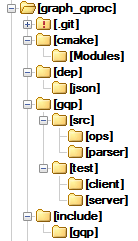
\includegraphics[scale=1]{structure}
\caption{Дерево файлов проекта}
\label{fig:structure}
\end{figure}

